\section{Learning \& Training Dynamics}

\subsection*{Q: What is the role of Batch Normalization (BN) in training neural networks?}
\textbf{Batch normalization} normalizes the input of each layer to have zero mean and unit variance across a mini-batch. This reduces internal co-variate shift (changes in the distribution of layer inputs during training), speeds up convergence, and stabilizes activation distributions and gradients.

\subsection*{Q: Why are learnable scale and shift parameters (\(\gamma, \beta\)) included in BN?}
BN restricts the distribution of outputs into the same fixed distribution (mean=0, variance=1), which prevents the network from learning the optimal scale and bias. These parameters allow the network to undo the normalization if necessary, preserving representational power after the input is normalized.

\subsection*{Q: Where should BN be applied in a neural network?}
\textbf{Batch normalization} is typically applied after the affine transformation (like a linear or convolutional layer) and before the activation function such as ReLU. BN normalizes the pre-activation values which stabilizes the distribution before they pass through nonlinearities, which keeps gradients flowing smoothly during backpropagation. BN, typically, is not applied to the output layers.

\subsection*{Q: What are the limitations of BN with small batch sizes?}
Small batch sizes lead to noisy estimates of the mean and variance, which can destabilize training and degrade performance. This may result in issues such as batch-wise overfitting or jittery parameter updates. Additionally, Batch Normalization loses much of its regularization effect when batch statistics become unreliable. In practice, a "small batch" typically refers to fewer than 32 samples per batch per device.

\subsection*{Q: How does batch normalization work during inference?}
During inference, batch normalization (BN) uses the running averages of the mean and variance computed during training, rather than calculating them from the current batch of data. This ensures deterministic outputs regardless of batch size. However, the outputs during inference may differ slightly from those during training due to the shift from batch-wise statistics to running estimates.

\subsection*{Q: How do BatchNorm, LayerNorm, GroupNorm, and InstanceNorm compare?}
\begin{figure}[H]
	\centering
	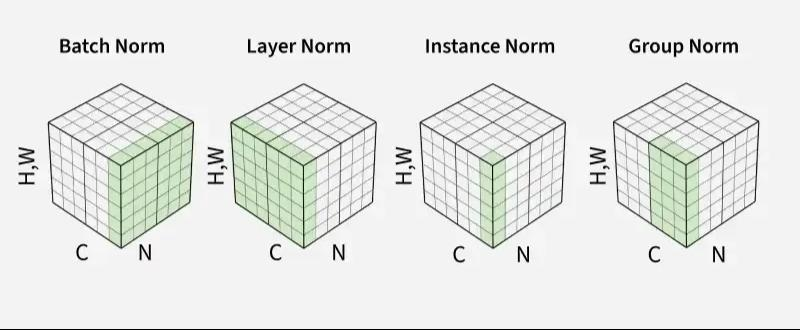
\includegraphics[width=0.8\textwidth]{norms.jpg}
	\caption{Source: \textit{https://www.geeksforgeeks.org/deep-learning/what-is-group-normalization/}}
\end{figure}
\begin{itemize}
	\item \textbf{Batch Normalization (BatchNorm)}: BatchNorm normalizes inputs across the batch dimension for each feature channel. It works well with large batch sizes and helps stabilize and accelerate training, but it can perform poorly with small batches and behaves differently during inference.
	\item \textbf{Layer Normalization (LayerNorm)}: LayerNorm normalizes across all feature dimensions within a single data sample. It is independent of batch size (robust for small batches) and is commonly used in architectures like Transformers and RNNs, but it tends to be less effective in convolutional neural networks.
	\item \textbf{Group Normalization (GroupNorm)}: GroupNorm divides channels into smaller groups and normalizes within each group. It performs consistently regardless of batch size and is particularly effective for convolutional models, though it requires tuning the number of groups (e.g., num groups=32).
	\item \textbf{Instance Normalization (InstanceNorm)}: InstanceNorm normalizes each individual sample and channel across spatial dimensions. It is widely used in style transfer applications as it helps remove instance-specific contrast information, but it may hurt performance in classification tasks where style information is important.
\end{itemize}

In summary, the choice of normalization method depends heavily on the task and batch size. For convolutional neural networks (CNNs) trained on large datasets like ImageNet, \textbf{BatchNorm} is the preferred choice. In scenarios with small batch sizes, such as object detection or segmentation, \textbf{GroupNorm} is typically more stable and effective. For natural language processing (NLP) and Transformer-based architectures, \textbf{LayerNorm} is widely used due to its batch-size independence. Finally, in style transfer or generative adversarial networks (GANs), \textbf{InstanceNorm} is favored for its ability to discard contrast and style-specific information.

\subsection*{Q: What are the differences between SGD and Adam?}
\textbf{SGD} uses a fixed or scheduled learning rate and is memory-efficient. \textbf{Adam} adapts learning rates for each parameter and converges faster but may overfit.

\subsection*{Q: What is the role of momentum in SGD?}
\textbf{Momentum} accumulates past gradients to smooth updates and accelerate convergence, especially in consistent gradient directions, and dampen oscillations caused by noisy gradients.

\subsection*{Q: How can overfitting be reduced in machine learning models?}
Techniques include collecting more data (e.g., data augmentation), regularization (e.g., weight decay, dropout, L1/L2 regularization), early stopping, learning rate scheduling, model simplification, and model ensembling.

\subsection*{Q: What is the difference between L1 and L2 regularization?}
\textbf{L1} adds absolute value penalties, leading to sparse models. \textbf{L2} adds squared penalties, keeping weights small but non-zero.

\subsection*{Q: How does dropout work?}
\textbf{Dropout} is a regularization technique that randomly deactivates (or "drops") neurons during training with a specified probability. This prevents the network from becoming overly reliant on specific neurons and encourages redundancy in learned representations, which helps reduce overfitting.

A high dropout rate increases regularization, which may cause the model to underfit if too much information is lost. Conversely, a low dropout rate provides weaker regularization, which may lead to overfitting if the model memorizes training data.

\subsection*{Q: Why does dropout improve generalization?}
\textbf{Dropout} acts like training many sub-networks and adds noise to the training process, which reduces overfitting and improves generalization.

\subsection*{Q: What are common activation functions and their pros/cons?}
\begin{figure}[H]
	\centering
	\includegraphics[width=0.8\textwidth]{activation.png}
	\caption{Source: \textit{https://blog.devops.dev/exploring-activation-functions-in-deep-learning-properties-derivatives-and-impact-on-model-7585aad8a757}.}
\end{figure}

\begin{itemize}
	\item \textbf{Sigmoid}: The sigmoid function is easy to interpret as it outputs values in (0, 1), but it may suffer from the vanishing gradient problem, especially at extreme input values.
	      \[
		      \sigma(x) = \frac{1}{1 + e^{-x}}
	      \]

	\item \textbf{Tanh}: The tanh function is zero-centered and ranges (-1, 1), which can help with optimization, but like the sigmoid function, it also experiences vanishing gradients.
	      \[
		      \tanh(x) = \frac{e^x - e^{-x}}{e^x + e^{-x}}
	      \]

	\item \textbf{ReLU}: The ReLU (Rectified Linear Unit) function is computationally efficient and helps create sparse representations, but it can suffer from the "dying ReLU" problem, where neurons become inactive.
	      \[
		      \text{ReLU}(x) = \max(0, x)
	      \]

	\item \textbf{Leaky ReLU}: The Leaky ReLU addresses the dying ReLU issue by allowing a small, non-zero gradient when the unit is not active, improving learning stability.
	      \[
		      \text{LeakyReLU}(x) =
		      \begin{cases}
			      x        & \text{if } x \geq 0 \\
			      \alpha x & \text{if } x < 0
		      \end{cases}
	      \]
	      where \( \alpha \) is a small positive constant (typically \( \alpha = 0.01 \)).

	\item \textbf{Softmax}: The softmax function converts logits into a probability distribution over classes, making it suitable for multi-class classification problems.
	      \[
		      \text{Softmax}(z_i) = \frac{e^{z_i}}{\sum_{j=1}^{C} e^{z_j}}
	      \]
	      where \( z_i \) is the logit for class \( i \), and \( C \) is the number of classes.
\end{itemize}

\subsection*{Q: When should you use Sigmoid vs Softmax?}
Use Sigmoid for binary or multi-label tasks. Use Softmax for mutually exclusive multi-class classification.
